\documentclass[twoside]{book}

% Packages required by doxygen
\usepackage{calc}
\usepackage{doxygen}
\usepackage{graphicx}
\usepackage[utf8]{inputenc}
\usepackage{makeidx}
\usepackage{multicol}
\usepackage{multirow}
\usepackage{textcomp}
\usepackage[table]{xcolor}

% Font selection
\usepackage[T1]{fontenc}
\usepackage{mathptmx}
\usepackage[scaled=.90]{helvet}
\usepackage{courier}
\usepackage{amssymb}
\usepackage{sectsty}
\renewcommand{\familydefault}{\sfdefault}
\allsectionsfont{%
  \fontseries{bc}\selectfont%
  \color{darkgray}%
}
\renewcommand{\DoxyLabelFont}{%
  \fontseries{bc}\selectfont%
  \color{darkgray}%
}

% Page & text layout
\usepackage{geometry}
\geometry{%
  a4paper,%
  top=2.5cm,%
  bottom=2.5cm,%
  left=2.5cm,%
  right=2.5cm%
}
\tolerance=750
\hfuzz=15pt
\hbadness=750
\setlength{\emergencystretch}{15pt}
\setlength{\parindent}{0cm}
\setlength{\parskip}{0.2cm}
\makeatletter
\renewcommand{\paragraph}{%
  \@startsection{paragraph}{4}{0ex}{-1.0ex}{1.0ex}{%
    \normalfont\normalsize\bfseries\SS@parafont%
  }%
}
\renewcommand{\subparagraph}{%
  \@startsection{subparagraph}{5}{0ex}{-1.0ex}{1.0ex}{%
    \normalfont\normalsize\bfseries\SS@subparafont%
  }%
}
\makeatother

% Headers & footers
\usepackage{fancyhdr}
\pagestyle{fancyplain}
\fancyhead[LE]{\fancyplain{}{\bfseries\thepage}}
\fancyhead[CE]{\fancyplain{}{}}
\fancyhead[RE]{\fancyplain{}{\bfseries\leftmark}}
\fancyhead[LO]{\fancyplain{}{\bfseries\rightmark}}
\fancyhead[CO]{\fancyplain{}{}}
\fancyhead[RO]{\fancyplain{}{\bfseries\thepage}}
\fancyfoot[LE]{\fancyplain{}{}}
\fancyfoot[CE]{\fancyplain{}{}}
\fancyfoot[RE]{\fancyplain{}{\bfseries\scriptsize Generated on Thu Jan 14 2016 13\-:40\-:33 for My Project by Doxygen }}
\fancyfoot[LO]{\fancyplain{}{\bfseries\scriptsize Generated on Thu Jan 14 2016 13\-:40\-:33 for My Project by Doxygen }}
\fancyfoot[CO]{\fancyplain{}{}}
\fancyfoot[RO]{\fancyplain{}{}}
\renewcommand{\footrulewidth}{0.4pt}
\renewcommand{\chaptermark}[1]{%
  \markboth{#1}{}%
}
\renewcommand{\sectionmark}[1]{%
  \markright{\thesection\ #1}%
}

% Indices & bibliography
\usepackage{natbib}
\usepackage[titles]{tocloft}
\setcounter{tocdepth}{3}
\setcounter{secnumdepth}{5}
\makeindex

% Hyperlinks (required, but should be loaded last)
\usepackage{ifpdf}
\ifpdf
  \usepackage[pdftex,pagebackref=true]{hyperref}
\else
  \usepackage[ps2pdf,pagebackref=true]{hyperref}
\fi
\hypersetup{%
  colorlinks=true,%
  linkcolor=blue,%
  citecolor=blue,%
  unicode%
}

% Custom commands
\newcommand{\clearemptydoublepage}{%
  \newpage{\pagestyle{empty}\cleardoublepage}%
}


%===== C O N T E N T S =====

\begin{document}

% Titlepage & ToC
\hypersetup{pageanchor=false}
\pagenumbering{roman}
\begin{titlepage}
\vspace*{7cm}
\begin{center}%
{\Large My Project }\\
\vspace*{1cm}
{\large Generated by Doxygen 1.8.6}\\
\vspace*{0.5cm}
{\small Thu Jan 14 2016 13:40:33}\\
\end{center}
\end{titlepage}
\clearemptydoublepage
\tableofcontents
\clearemptydoublepage
\pagenumbering{arabic}
\hypersetup{pageanchor=true}

%--- Begin generated contents ---
\chapter{Card-\/\-Shuffeling}
\label{index}\hypertarget{index}{}\begin{DoxyParagraph}{}
Das Card-\/\-Shuffeling-\/\-Tool dient zum Vorzeigen einer Doxygen-\/\-Dokumentationen. Das Programm wurde absichtlich mit einem Overhead an Klassen und Funktionen geschrieben, um das Verhalten von Doxygen zeigen zu können. 
\end{DoxyParagraph}
\begin{DoxyParagraph}{}
Das Programm Card-\/\-Shuffeling dient zur zufälligen Verteilung von mehreren Kartendecks (32 Karten, 4 Farben a 8 Karten) an eine eingestellte Zahl an Spielern. Es soll statistisch Auswerten, wie häufig ein \char`\"{}blanker Zehner\char`\"{} in Abhängigkeit der Anzahl der Decks und Spieler auftritt. 
\end{DoxyParagraph}

\chapter{Class Index}
\section{Class List}
Here are the classes, structs, unions and interfaces with brief descriptions\-:\begin{DoxyCompactList}
\item\contentsline{section}{\hyperlink{struct_c_a_r_d}{C\-A\-R\-D} \\*\hyperlink{struct_c_a_r_d}{C\-A\-R\-D} ist ein Struct zur Darstellung von Karten }{\pageref{struct_c_a_r_d}}{}
\item\contentsline{section}{\hyperlink{classdeck}{deck} \\*Die Klasse deck repräsentiert ein gewöhnliches Kartendeck }{\pageref{classdeck}}{}
\item\contentsline{section}{\hyperlink{classmatch}{match} \\*Die Klasse \hyperlink{classmatch}{match} generiert eine Rund eines Kartenspiels an welchem \#\-P\-L\-A\-Y\-E\-R\-S Spieler teilnehmen und \#\-S\-I\-Z\-E\-\_\-\-D\-E\-C\-K\-S Decks verwendet werden }{\pageref{classmatch}}{}
\item\contentsline{section}{\hyperlink{classplayer}{player} \\*Die Klasse \hyperlink{classplayer}{player} stellt einen Teilernehmer des Kartenspiels \hyperlink{classmatch}{match} dar }{\pageref{classplayer}}{}
\end{DoxyCompactList}

\chapter{File Index}
\subsection{Auflistung der Dateien}
Hier folgt die Aufzählung aller Dateien mit einer Kurzbeschreibung\-:\begin{DoxyCompactList}
\item\contentsline{section}{\hyperlink{main_8cpp}{main.\-cpp} \\*Initialise cards matches }{\pageref{df/d0a/main_8cpp}}{}
\item\contentsline{section}{\hyperlink{match_8cpp}{match.\-cpp} }{\pageref{d1/d30/match_8cpp}}{}
\item\contentsline{section}{\hyperlink{match_8h}{match.\-h} }{\pageref{d1/d61/match_8h}}{}
\item\contentsline{section}{\hyperlink{player_8cpp}{player.\-cpp} }{\pageref{db/d80/player_8cpp}}{}
\item\contentsline{section}{\hyperlink{player_8h}{player.\-h} \\*Datie zur Verwaltung der Klasse(n) \hyperlink{classplayer}{player} }{\pageref{d3/d62/player_8h}}{}
\item\contentsline{section}{\hyperlink{set_8cpp}{set.\-cpp} }{\pageref{d0/d6e/set_8cpp}}{}
\item\contentsline{section}{\hyperlink{set_8h}{set.\-h} }{\pageref{d4/d13/set_8h}}{}
\end{DoxyCompactList}

\chapter{Class Documentation}
\hypertarget{struct_c_a_r_d}{\section{C\-A\-R\-D Struct Reference}
\label{struct_c_a_r_d}\index{C\-A\-R\-D@{C\-A\-R\-D}}
}


\hyperlink{struct_c_a_r_d}{C\-A\-R\-D} ist ein Struct zur Darstellung von Karten.  




{\ttfamily \#include $<$set.\-h$>$}

\subsection*{Public Attributes}
\begin{DoxyCompactItemize}
\item 
\hypertarget{struct_c_a_r_d_a36f0e6c29177b3e38a73a17c57d2f0ac}{int {\bfseries number}}\label{struct_c_a_r_d_a36f0e6c29177b3e38a73a17c57d2f0ac}

\item 
\hypertarget{struct_c_a_r_d_a931664b6380e876a72b664225ddfe20d}{int {\bfseries color}}\label{struct_c_a_r_d_a931664b6380e876a72b664225ddfe20d}

\end{DoxyCompactItemize}


\subsection{Detailed Description}
\hyperlink{struct_c_a_r_d}{C\-A\-R\-D} ist ein Struct zur Darstellung von Karten. 

Dabei gibt Number die Nummer (7, 8, 9, 10, K, O, U, A) an und color steht für die I\-D einer Farbe. 

The documentation for this struct was generated from the following file\-:\begin{DoxyCompactItemize}
\item 
set.\-h\end{DoxyCompactItemize}

\hypertarget{classdeck}{\section{deck Class Reference}
\label{classdeck}\index{deck@{deck}}
}


Die Klasse deck repräsentiert ein gewöhnliches Kartendeck.  




{\ttfamily \#include $<$set.\-h$>$}

\subsection*{Public Member Functions}
\begin{DoxyCompactItemize}
\item 
\hypertarget{classdeck_a2ff8465ba7b13201bdf650fe461b442e}{\hyperlink{classdeck_a2ff8465ba7b13201bdf650fe461b442e}{deck} ()}\label{classdeck_a2ff8465ba7b13201bdf650fe461b442e}

\begin{DoxyCompactList}\small\item\em \hyperlink{classdeck_a2ff8465ba7b13201bdf650fe461b442e}{deck\-::deck} Füllt ein Deck mit \#\-C\-O\-L\-O\-R\-S$\ast$\#\-N\-U\-M\-B\-E\-R\-S Karten auf. \end{DoxyCompactList}\item 
\hypertarget{classdeck_a26cfcf4196728cde8b904dbcf63bc815}{std\-::vector$<$ \hyperlink{struct_c_a_r_d}{C\-A\-R\-D} $>$ {\bfseries get\-Cards} (void)}\label{classdeck_a26cfcf4196728cde8b904dbcf63bc815}

\item 
\hypertarget{classdeck_a3a190c2877d3822b7379d6a9fa2c050b}{int {\bfseries is\-Empty} ()}\label{classdeck_a3a190c2877d3822b7379d6a9fa2c050b}

\item 
\hyperlink{struct_c_a_r_d}{C\-A\-R\-D} \hyperlink{classdeck_a8e33dbdafe69c55d968526d9543245ec}{get\-Random\-Card} ()
\begin{DoxyCompactList}\small\item\em \hyperlink{classdeck_a8e33dbdafe69c55d968526d9543245ec}{deck\-::get\-Random\-Card} zieht eine zufällige Karte auf dem Kartendeck und entfernt diese. \end{DoxyCompactList}\end{DoxyCompactItemize}


\subsection{Detailed Description}
Die Klasse deck repräsentiert ein gewöhnliches Kartendeck. 

Hier dient sie um größere Kartendecks innerhalb eines Matches zusammen zu stellen. 

\subsection{Member Function Documentation}
\hypertarget{classdeck_a8e33dbdafe69c55d968526d9543245ec}{\index{deck@{deck}!get\-Random\-Card@{get\-Random\-Card}}
\index{get\-Random\-Card@{get\-Random\-Card}!deck@{deck}}
\subsubsection[{get\-Random\-Card}]{\setlength{\rightskip}{0pt plus 5cm}{\bf C\-A\-R\-D} deck\-::get\-Random\-Card (
\begin{DoxyParamCaption}
{}
\end{DoxyParamCaption}
)}}\label{classdeck_a8e33dbdafe69c55d968526d9543245ec}


\hyperlink{classdeck_a8e33dbdafe69c55d968526d9543245ec}{deck\-::get\-Random\-Card} zieht eine zufällige Karte auf dem Kartendeck und entfernt diese. 

\begin{DoxyReturn}{Returns}
gezogene Karte. 
\end{DoxyReturn}


The documentation for this class was generated from the following files\-:\begin{DoxyCompactItemize}
\item 
set.\-h\item 
set.\-cpp\end{DoxyCompactItemize}

\hypertarget{classmatch}{\section{match Class Reference}
\label{classmatch}\index{match@{match}}
}


Die Klasse \hyperlink{classmatch}{match} generiert eine Rund eines Kartenspiels an welchem \#\-P\-L\-A\-Y\-E\-R\-S Spieler teilnehmen und \#\-S\-I\-Z\-E\-\_\-\-D\-E\-C\-K\-S Decks verwendet werden.  




{\ttfamily \#include $<$match.\-h$>$}

\subsection*{Public Member Functions}
\begin{DoxyCompactItemize}
\item 
\hypertarget{classmatch_a324c10417644283bb7101859392ed252}{\hyperlink{classmatch_a324c10417644283bb7101859392ed252}{match} ()}\label{classmatch_a324c10417644283bb7101859392ed252}

\begin{DoxyCompactList}\small\item\em \hyperlink{classmatch_a324c10417644283bb7101859392ed252}{match\-::match} Erstellt das Masterdeck aus bestehenden Decks und verteilt die Karten an alle Spieler. \end{DoxyCompactList}\end{DoxyCompactItemize}


\subsection{Detailed Description}
Die Klasse \hyperlink{classmatch}{match} generiert eine Rund eines Kartenspiels an welchem \#\-P\-L\-A\-Y\-E\-R\-S Spieler teilnehmen und \#\-S\-I\-Z\-E\-\_\-\-D\-E\-C\-K\-S Decks verwendet werden. 

Dabei werden an alle Teilnehmer gleich viele Karten aus den zuvor erstellten Decks zufällig verteilt. 

The documentation for this class was generated from the following files\-:\begin{DoxyCompactItemize}
\item 
match.\-h\item 
match.\-cpp\end{DoxyCompactItemize}

\hypertarget{classplayer}{\section{player Class Reference}
\label{classplayer}\index{player@{player}}
}


Die Klasse \hyperlink{classplayer}{player} stellt einen Teilernehmer des Kartenspiels \hyperlink{classmatch}{match} dar.  




{\ttfamily \#include $<$player.\-h$>$}

\subsection*{Public Member Functions}
\begin{DoxyCompactItemize}
\item 
\hypertarget{classplayer_a97de83bce15f880241f561b55b016b02}{\hyperlink{classplayer_a97de83bce15f880241f561b55b016b02}{player} ()}\label{classplayer_a97de83bce15f880241f561b55b016b02}

\begin{DoxyCompactList}\small\item\em \hyperlink{classplayer_a97de83bce15f880241f561b55b016b02}{player\-::player} \end{DoxyCompactList}\item 
void \hyperlink{classplayer_a7ee9bffda2073c5ffa036fd978cea86d}{get\-Card} (\hyperlink{struct_c_a_r_d}{C\-A\-R\-D} card)
\begin{DoxyCompactList}\small\item\em \hyperlink{classplayer_a7ee9bffda2073c5ffa036fd978cea86d}{player\-::get\-Card} deals a card to the player \end{DoxyCompactList}\item 
\hypertarget{classplayer_a3dc68b6bb16cc8cb5d2a8bdbe9979bda}{void \hyperlink{classplayer_a3dc68b6bb16cc8cb5d2a8bdbe9979bda}{print\-Cards} ()}\label{classplayer_a3dc68b6bb16cc8cb5d2a8bdbe9979bda}

\begin{DoxyCompactList}\small\item\em \hyperlink{classplayer_a3dc68b6bb16cc8cb5d2a8bdbe9979bda}{player\-::print\-Cards} listet alle Handkarten des Spielers auf. \end{DoxyCompactList}\end{DoxyCompactItemize}


\subsection{Detailed Description}
Die Klasse \hyperlink{classplayer}{player} stellt einen Teilernehmer des Kartenspiels \hyperlink{classmatch}{match} dar. 

Der Spieler kann Karten annehmen und seine Handkarten printen. 

\subsection{Member Function Documentation}
\hypertarget{classplayer_a7ee9bffda2073c5ffa036fd978cea86d}{\index{player@{player}!get\-Card@{get\-Card}}
\index{get\-Card@{get\-Card}!player@{player}}
\subsubsection[{get\-Card}]{\setlength{\rightskip}{0pt plus 5cm}void player\-::get\-Card (
\begin{DoxyParamCaption}
\item[{{\bf C\-A\-R\-D}}]{card}
\end{DoxyParamCaption}
)}}\label{classplayer_a7ee9bffda2073c5ffa036fd978cea86d}


\hyperlink{classplayer_a7ee9bffda2073c5ffa036fd978cea86d}{player\-::get\-Card} deals a card to the player 


\begin{DoxyParams}{Parameters}
{\em card} & which is dealed to the player \\
\hline
\end{DoxyParams}


The documentation for this class was generated from the following files\-:\begin{DoxyCompactItemize}
\item 
\hyperlink{player_8h}{player.\-h}\item 
player.\-cpp\end{DoxyCompactItemize}

\chapter{File Documentation}
\hypertarget{main_8cpp}{\section{main.\-cpp File Reference}
\label{main_8cpp}\index{main.\-cpp@{main.\-cpp}}
}


Initialise cards matches.  


{\ttfamily \#include $<$iostream$>$}\\*
{\ttfamily \#include \char`\"{}match.\-h\char`\"{}}\\*
\subsection*{Functions}
\begin{DoxyCompactItemize}
\item 
\hypertarget{main_8cpp_ae66f6b31b5ad750f1fe042a706a4e3d4}{int {\bfseries main} ()}\label{main_8cpp_ae66f6b31b5ad750f1fe042a706a4e3d4}

\end{DoxyCompactItemize}


\subsection{Detailed Description}
Initialise cards matches. \begin{DoxyAuthor}{Author}
Andreas Conrads (\href{mailto:aco@cadsoft.de}{\tt aco@cadsoft.\-de}) 
\end{DoxyAuthor}
\begin{DoxyDate}{Date}
Jan, 2016 Initialise and excecute \#\-G\-A\-M\-E\-S card matches. 
\end{DoxyDate}

\hypertarget{player_8h}{\subsection{player.\-h-\/\-Dateireferenz}
\label{player_8h}\index{player.\-h@{player.\-h}}
}


Datie zur Verwaltung der Klasse(n) \hyperlink{classplayer}{player}.  


{\ttfamily \#include $<$vector$>$}\\*
{\ttfamily \#include $<$iostream$>$}\\*
{\ttfamily \#include \char`\"{}set.\-h\char`\"{}}\\*
Include-\/\-Abhängigkeitsdiagramm für player.\-h\-:\nopagebreak
\begin{figure}[H]
\begin{center}
\leavevmode
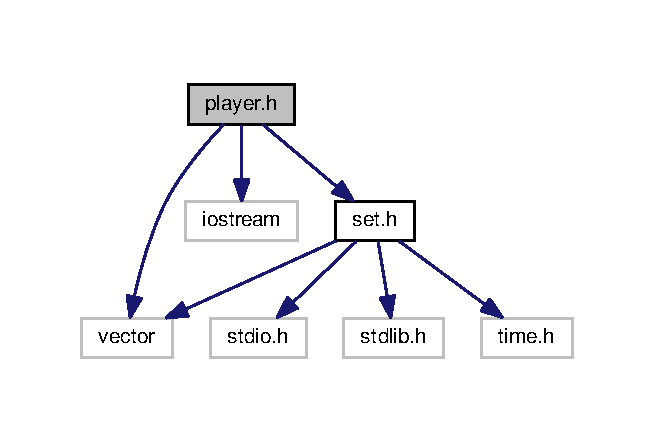
\includegraphics[width=315pt]{d1/d98/player_8h__incl}
\end{center}
\end{figure}
\subsubsection*{Klassen}
\begin{DoxyCompactItemize}
\item 
class \hyperlink{classplayer}{player}
\begin{DoxyCompactList}\small\item\em Die Klasse \hyperlink{classplayer}{player} stellt einen Teilernehmer des Kartenspiels \hyperlink{classmatch}{match} dar. \end{DoxyCompactList}\end{DoxyCompactItemize}


\subsubsection{Ausführliche Beschreibung}
Datie zur Verwaltung der Klasse(n) \hyperlink{classplayer}{player}. \begin{DoxyAuthor}{Autor}
Andreas Conrads 
\end{DoxyAuthor}
\begin{DoxyDate}{Datum}
2016/01/08 
\end{DoxyDate}


Definiert in Datei \hyperlink{player_8h_source}{player.\-h}.


%--- End generated contents ---

% Index
\newpage
\phantomsection
\addcontentsline{toc}{chapter}{Index}
\printindex

\end{document}
